\documentclass[12pt]{article}

\usepackage[T1]{fontenc}
\usepackage[utf8]{inputenc}
\usepackage{algorithm} %for numbered code
\usepackage{algorithmic} %for pseudocode
\usepackage{times}
\usepackage{epsfig}
\usepackage{graphicx}
\usepackage{amsmath}
\usepackage{amssymb}
\usepackage{color, soul} 	%for highlighting
\usepackage{listings} 		%for writing code
\lstset{
basicstyle=\small\ttfamily,
columns=flexible,
breaklines=true
}
\usepackage[margin=1in]{geometry} %for margins
\setlength{\parskip}{12pt plus3pt minus3pt} %for paragraph spacing

\setcounter{page}{1}
\begin{document}

\begin{titlepage}

\title{Space Brain - Investigating the Suitability of FPGA based Convolutional Neural Network for Space Applications}
\author{Jacobus (Jukka) Johannes Hertzog}
\def\supervisor{Dr. Felix Winterstein}
\def\secondmarker{Dr. David Thomas}
\def\course{EE4T}
\def\cid{00828711}

\setlength{\parindent}{0pt}
\setlength{\parskip}{0pt}
\fontfamily{phv}\selectfont
{
\large
\raggedright
Imperial College London\\[17pt]
Department of Electrical and Electronic Engineering\\[17pt]
Final Year Project Report 2017\\[17pt]
}
\rule{\columnwidth}{3pt}
\vfill
\centering
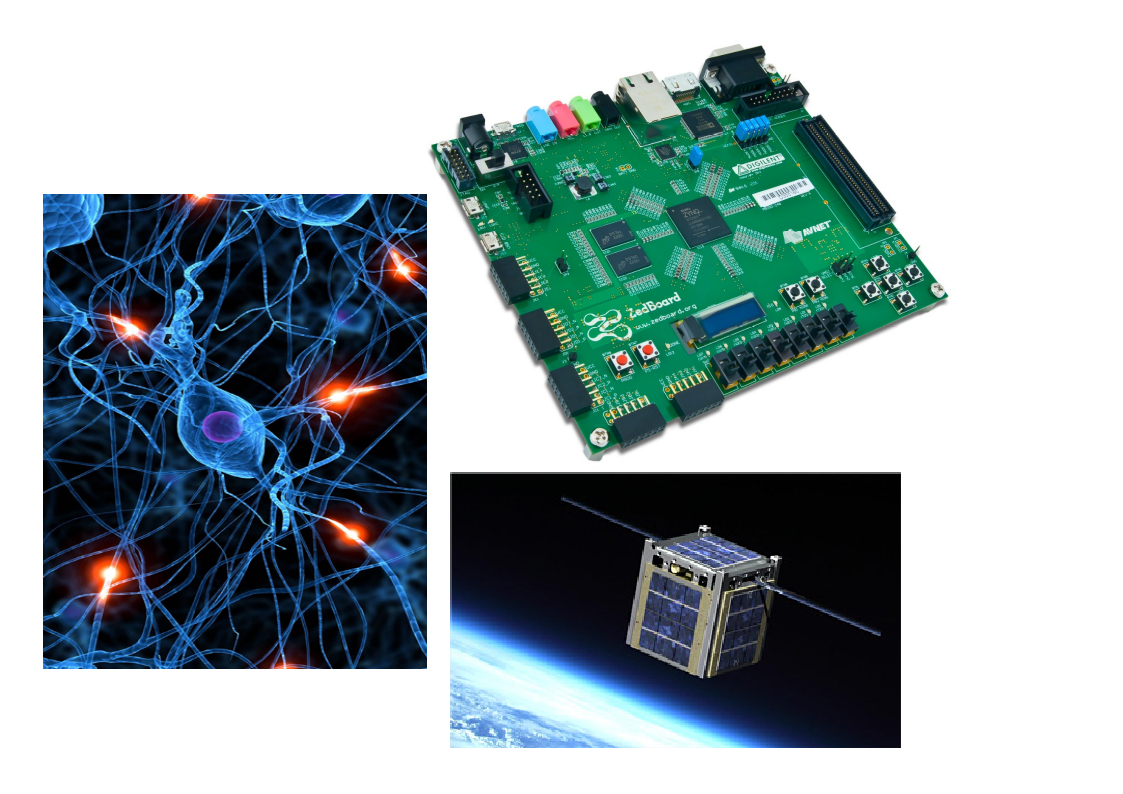
\includegraphics[width=\columnwidth,keepaspectratio]{../figures/frontCover}
\vfill
\setlength{\tabcolsep}{0pt}


\makeatletter
\begin{tabular}{p{40mm}p{\dimexpr\columnwidth-40mm}}
Project Title: & \textbf{\@title} \\[12pt]
Student: & \textbf{\@author} \\[12pt]
CID: & \textbf{\cid} \\[12pt]
Course: & \textbf{\course} \\[12pt]
Project Supervisor: & \textbf{\supervisor} \\[12pt]
Second Marker: & \textbf{\secondmarker} \\
\end{tabular}
\end{titlepage}

\begin{abstract}
Over the last decade, advancements in the design of Convolutional Neural Networks (CNNs) have led to significant improvements in the accuracy of image classification systems. A potential application of a CNN image classifier would be  processing data on board a satellite. In such a situation, with limited power and computational resources, it would be beneficial to make use of an FPGA in order to alleviate the resource demands of the computationally expensive CNN. However, FPGAs are sensitive to ionizing radiation, and at orbital altitudes, the high radiation environment can induce a variety of errors in the FPGA fabric, casting doubt on the suitability of a commercial FPGA for CNN applications in space.

This project implements an FPGA based CNN, and simulates radiation-induced errors. These results are analyzed to determine the impact on the system’s performance. \hl{[The tests are yet to be performed, and as such, this part of the abstract is not yet completed.]} The implementation target platform is the ZedBoard Zynq-7000 ARM/FPGA SoC. The  hardware and software portions of the embedded system are both implemented  using the Xilinx SDSoC development environment.
\end{abstract}

\newpage

\renewcommand{\abstractname}{Acknowledgements}
\begin{abstract}
\hl{TODO}
\end{abstract}

\newpage

\tableofcontents

\newpage

\section{Introduction}
\label{sec:Intro}
\vspace{-12pt}

Inspired by the structure of the optical nervous system in animals, a neural network is made up of layers of artificial neurons that recognise certain features from the input data. The concept of an artificial neural network was first introduced in 1980 \cite{neocognitron}, and driven by increases in computing power and a growth in machine learning applications, neural networks have become very powerful tools. In the last decade, the development of Convolutional Neural Networks (CNNs) has lead to great advancements in image classification accuracy.

CNNs are a powerful Deep Learning tool that can be used to solve extremely complex computational problems. In particular, they have gained popularity in image classification applications \cite{ImageNetChallenge}. Other popular applications within machine vision include video classification, face detection and gesture recognition. They are also being used in a wide range of other fields including speech recognition, natural language processing and text classification.

However, whilst achieving exceptional performance, CNNs are extremely computation and resource heavy. Typically, they will be implemented on large servers or on GPU based systems to accommodate the need for computational power. As a result, implementing them on embedded systems, which typically have very limited resources, presents many challenges. A promising solution to this problem is the use of an FPGA, which provide a very high computational efficiency with low power usage, in addition to other benefits.

Now suppose that the FPGA based CNN will be implemented on a satellite. In orbit, the satellite will be exposed to intense radiation, and as a result, errors will be produced on the radiation-sensitive FPGA. Before such a satellite can be designed and launched, it is important to know how these errors would affect the performance of the CNN, and if the CNN design could be modified to mitigate the impact of these errors. Therefore, the aim of this project is to implement a CNN on an FPGA-based system, and then to investigate the suitability of this system for space applications.

\subsection{Project Motivation}
\label{sec:Intro-ProjectMotivation}
\vspace{-12pt}

\begin{itemize}
\item \hl{Describe need for analysis of impact of SEUs}
\end{itemize}

\vspace{-12pt}
\subsection{Report Structure}
\label{sec:Intro-Structure}
\vspace{-12pt}

\textbf{Section \ref{sec:Background} - Background:} In order to guarantee that the reader has the contextual knowledge required to understand the project, this section will describe the Target Platform, High Level Synthesis, and CNNs. FPGA implementations of CNNs and the difficulties of using FPGAs in satellites will also be explored.\\
\\
\textbf{Section \ref{sec:ProjSpec} - Project Specification:} This section details the project requirements that should be met by the final system.\\
\\
\textbf{Section \ref{sec:Design} - Design:} The decisions taken in the design process are described and explained in this section. The high level design is described, as well important aspects of the low level design.\\
\\
\textbf{Section \ref{sec:Imp} - Implementation:} This section illustrate how the system was implemented, aiming to provide the reader with an understanding of the development process.\\
\\
\textbf{Section \ref{sec:Test} - Testing:} The testing methodology used to verify various components of the system is detailed in this section.\\
\\
\textbf{Section \ref{sec:Eval} - Evaluation:} The focus of this section is the result of the investigation, including an evaluation of the system's performance.\\
\\
\textbf{Section \ref{sec:Conclusion} - Conclusion and Future Work:} This section will summarize the results of the project, highlight areas for improvement and further work, and present concluding remarks.\\

\newpage

\section{Background}
\label{sec:Background}
\vspace{-12pt}

This section will provide some details and information that will provide context to the project, and will be useful for understanding key concepts in the rest of the report. The High Level Synthesis tools, CNN structures, FPGA implementations of CNNs, and the issues surrounding the use of FPGAs in space will all be discussed.

\subsection{Target Platform}
\label{sec:Background-TargetPlatform}
\vspace{-12pt}

The hardware used in this project is a product from Xilinx called a Zedboard, a development board for the Zynq-7000 System On a Chip (SoC). This board was chosen because of its useful hardware features and its integrated support for valuable Xilinx proprietary tools. These tools include High Level Synthesis systems, SoC design tools and the Soft Error Mitigation IP core. The Zynq-7000 consists of a Xilinx FPGA as its Programmable Logic, and a dual-core Cortex-A9 ARM processor as its Processing System integrated together. The ARM processor facilitates easy control of the system, whilst the FPGA will be able to efficiently perform heavy computations.


\subsection{High Level Synthesis}
\label{sec:Background-HLS}
\vspace{-12pt}

Typically, digital circuits on reconfigurable hardware architectures, such as FPGAs, are designed using a Hardware Description Language (HDL) such as Verilog or VHDL. While these methods allow the designer to have a great level of control over the system, and can produce extremely efficient designs, the designer is forced to specify functionality at a very low level of abstraction, specifying cycle by cycle behaviour. Use of HDL tools requires hardware expertise and, when designing a complex system, makes for a long and cumbersome development process.

High Level Synthesis (HLS) tools are a  solution to this problem. An HLS tool is a piece of software which can interpret the desired behaviour of code written in a programming language like C or C++, and generate an HDL implementation of that behaviour, allowing the designer to work at a higher level of abstraction. This means that a software engineer can create FPGA designs without having to build up hardware expertise, allowing them to utilise the speed and efficiency of hardware designs. It also benefits hardware engineers, allowing them to design the system more quickly and reliably, facilitating the development of more complex systems \cite{HLS}. Popular HLS tools include academic, open-source software like LegUp, and commercial tools like Catapult-C and Xilinx's Vivado. In this project, the embedded system will be designed using SDSoC from Xilinx, which utilises Vivado HLS to produce a configuration for the Programmable Logic in the Zynq SoC.

\subsection{Convolutional Neural Networks}
\label{sec:Background-CNN}
\vspace{-12pt}

CNNs can be used to classify images in a forward inference process. But before using the CNN for any task, the CNN should be trained on a set of training data. The training of a CNN is often implemented on large servers with a significant computational capacity, with an enormous set of training data, or on a GPU when such a server is not available. For the embedded FPGA platform, this project will only focus on implementing and utilising the inference process of a CNN, and not on the training process.

A typical CNN consists of a number of layers that run in sequence. Convolution (CONV), activation function, pooling, and Fully Connected (FC) layers make up a typical CNN model, with CONV and FC being the most important. CONV and FC layers have parameters of called weights, which are set by the training process. These weights will determine which patterns each layer of the CNN will be activated by, and ultimately, what the CNN is able to recognise and classify. 

The first layer of a CNN reads an input image and outputs a series of feature maps. The input image will be three dimensional - the height and width of the image make up two dimensions, and colours make up the third layer. For an RGB image, the input will have a depth of 3. Then there will be CONV layers interspersed by activation function and pooling layers, which will make up most of the CNN. These layers will decompose the image into feature maps, varying from low-level features such as edges, lines, curves, etc., in the initial layers to high-level features in the deeper layers \cite{SudaFpgaAccelerator}. Each subsequent layer reads the feature maps generated by preceding layers and generates new feature maps at its output. Finally a classifier, consisting of at least one FC layer, reads the final feature maps and determines the probability of the input imaging belonging to each category of the training data. An example of a CNN model is shown in Figure \ref{fig:typicalCNN}.
\begin{figure}[h]
\centering
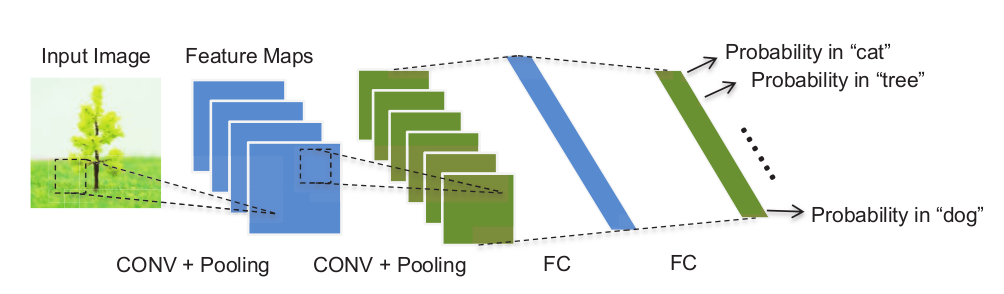
\includegraphics[width=0.75\textwidth]{../figures/typicalCnn}
\caption{A typical CNN structure from the feature map perspective \cite{embeddedFpgaCnn} \label{fig:typicalCNN}}
\end{figure}
\vspace{-12pt}

\subsubsection{Convolution Layer}
\label{sec:Background-CNN-Conv}
\vspace{-12pt}

The CONV layer takes a series of feature maps as input and convolves with convolutional kernels to obtain the output feature maps. It involves 3-dimensional multiply and accumulate operation of $N_{if}$ input features with $K\times K$ convolution kernels to get an output feature neuron value as shown in Equation \ref{eq:ConvLayer}
\begin{equation}
out(f_o,x,y)=\sum^{N_{if}}_{f_i=0} \sum^{K}_{k_x=0} \sum^{K}_{k_y=0} wt(f_o,f_i,k_x,k_y)\times in(f_i,x+k_x,y+k_y)
\label{eq:ConvLayer}
\end{equation}
where $out(f_o,x,y)$ and $in(f_i,x,y)$ represent the neurons at position $(x,y)$ in the feature maps $f_o$ and $f_i$, respectively and $wt(f_o,f_i,k_x,k_y)$ is the weights at position $(k_x,k_y)$ that gets convolved with input feature map $f_i$ to get the output feature map $f_o$ \cite{SudaFpgaAccelerator}.

\subsubsection{Activation Functions}
\label{sec:Background-CNN-Activation}
\vspace{-12pt}

CONV layers are followed by an activation function layer. This layer can be thought of as a decision, based on the output of the CONV layer, on to what extent each neuron in the next layer has been activated. The CONV layer output is a linear combination of the inputs and the weights at a position in the network, and role of the activation function is to produce a non-linear decision boundary. The commonly used activation functions in traditional neural networks are non-linear functions such as tanh and sigmoid, which require a longer training time in CNNs \cite{AlexNet}. Hence, Rectified Linear Unit (ReLU), defined as $y = max(x,0)$, has become the popular activation function among CNN models as it converges faster in training, and has less computational complexity than exponent functions in tanh and sigmoid, also aiding hardware design.

\subsubsection{Pooling Layer}
\label{sec:Background-CNN-Pool}
\vspace{-12pt}

Spatial pooling or sub-sampling is utilized to reduce the feature dimensions as we traverse deeper into the network. As shown in Equation \ref{eq:Pool}, pooling computes the maximum or average of neighbouring $K\times K$ neurons in the same feature map, which also provides a form of translational invariance \cite{PoolAnalysis}. The pooling layer helps abstract higher-level features without redundancy, as well as reducing the dimensionality of lower-level features without losing important information \cite{SudaFpgaAccelerator}.
\begin{equation}
out(f_o,x,y)=\underset{0\geqslant (k_x,k_y)<K}{max/average}(in(f_o,x+k_x,y+k_y))
\label{eq:Pool}
\end{equation}

\subsubsection{Fully Connected Layer}
\label{sec:Background-CNN-FC}
\vspace{-12pt}

An FC layer is a classification layer where all the input features $(N_{if})$ are connected to all of the output features $(N_{of})$ through synaptic weights $(wt)$. These are at the end of the CNN and perform the final classification, based on the features that have been recognised by the rest of the network. Each output neuron is the weighted summation of all the input neurons as shown in Equation \ref{eq:FullyConnected} \cite{SudaFpgaAccelerator}.
\begin{equation}
out(f_o)=\sum^{N_{if}}_{f_i=0}wt(f_o,f_i)\times in(f_i)
\label{eq:FullyConnected}
\end{equation}
The outputs of the inner-product layer traverse through ReLU based activation function to the next inner-product layer or directly to a Softmax function that converts them to probability in the range (0, 1). The final accuracy layer compares the labels of the top probabilities from softmax layer with the actual label and gives the accuracy of the CNN model \cite{SudaFpgaAccelerator}.

\subsection{FPGAs and CNN Implementations}
\label{sec:Background-FpgaCnnImpl}
\vspace{-12pt}

CNNs are computationally demanding and consume a lot of resources, and thus are difficult to implement on an embedded systems. FPGAs are the most promising platform for the implementation of an embedded CNN, due to their high computational efficiency and low power consumption. FPGAs are also more attractive than other digital hardware platforms, such as ASICS, because of their reconfigurability and fast development time, aided by HLS tools.

\subsubsection{Implementation Challenges}
\label{sec:Background-FpgaCnnImpl-Challenges}
\vspace{-12pt}

One of the main challenges faced by FPGA implementations is memory bandwidth. A typical CNN model may have more than 60 million weights, which requires over 200MB of memory when represented with a 32 bit number. A standard commercial FPGA does not have enough on-chip memory to store this volume of data, so external memory must be utilised. Having to transfer this information to the FPGA can introduce a computational bottleneck. However, these weights are used in CONV layers multiple times. Thus, the system can be optimised by reducing frequent memory access. Chen et. al achieves this with a tiling method and dedicated buffers for data re-use. Another approach, is data quantization, which is discussed below. By quantizing the 32-bit floating-point weights into 16-bit fixed-point values, the pressure on the memory system can be alleviated. Suda et al. performed a study on the optimal precisions to balance accuracy and efficiency. It was found that the best choices were 8-bit precision for CONV weights, 10-bit precision for FC weights, with less than 1\% compared accuracy loss compared to full precision weights \cite{SudaFpgaAccelerator}.

\subsubsection{FPGA CNN Accelerators}
\label{sec:Background-FpgaCnnImpl-Accel}
\vspace{-12pt}

An FPGA implementation of a CNN, intended to improve the speed and efficiency of the CNN computation, is referred to as an FPGA CNN accelerator. Most research into FPGA CNN accelerators has focussed on using hardware to accelerating the computation of the CONV layers. These layers typically make up around 90\% of the CNN's computational workload. The multiply and accumulate nature of the CONV layer's operation makes them ideal candidates for hardware acceleration, as FPGAs are able to perform these operations with great efficiency. 

FPGAs also provide flexibility to implement the CNNs with limited data precision \cite{SudaFpgaAccelerator}. Many CNN accelerators use 16-bit fixed-point numbers instead of floating-point numbers to represent weights and data \cite{ZhangFpgaAccelerator}\cite{ChenFpgaAccelerator}\cite{FarabetFpgaAccelerator}, especially because FPGAs. Using a shorter, fixed-point data representation can make significant reductions to the memory footprint and the use of computational resources. The CNN's data must be quantised in order for the fixed-point implementation to work, which will introduce a quantization error into the result. However, Chen et al. showed that using a 16-bit fixed-point implementation rather than a 32-bit fixed-point implementation only added an extra 0.26\% to the error rate when using the MNIST dataset.

\subsection{FPGAs and Space Applications}
\label{sec:Background-FPGAsAndSpaceApplications}
\vspace{-12pt}

\subsubsection{Single Event Upsets}
\label{sec:Background-FPGAsAndSpaceApplications-SEUs}
\vspace{-12pt}

Electronic circuits are sensitive to high-energy ionizing radiation, which can induce errors called Single Event Upsets (SEUs) \cite{SeuTutorial}. In space, this is a particular problem. The radiation shielding provided by the Earth's magnetosphere, and enjoyed by systems at lower altitudes, is no longer present, leaving systems open to radiation from a  variety of sources. A voltage pulse from an SEU can cause errors including altering digital values. SEU induced voltage pulses are problematic for all circuits in space, but the nature of reconfigurable circuits means that they are particularly vulnerable. These SEUs are typically manifested as a bit flip in a memory cell or a transient logic pulse in combinational logic. Habinc et al. describes three main categories of SEU \cite{SuitabilityGaisler}.

The first category is the configuration upset. FPGAs are configured by loading the configuration bitstream into an internal configuration memory. This memory controls the configurable logic elements and how they connect together. A configuration upset occurs when an SEU alters a value in the configuration memory, and thus changes the function of the configuration. 

The second category is the functional upsets in user logic are SEUs within the FPGA's logic. The FPGA's user logic cannot be tested through a readback of the configuration memory, because the logic contents will change as part of normal operation. These errors can cause transient glitches in combinatorial logic, and can upset sequential logic where the state of the system is vital to its function \cite{FTripleMR}.

The final category is the architectural upset. This is when an SEU occurs in the control elements of the FPGA, e.g. the configuration circuits or reset control \cite{SuitabilityGaisler}. This can have an enormous range of consequences. For example, an SEU in the reset control could cause the FPGA to be unintentionally reset and all state information would be lost due to the FPGA being reconfigured.

Architectural upsets are outside the scope of this project, but configuration and functional upsets will be investigated. This is explained in more detail in Section \ref{sec:ProjSpec-TestSpec}.

\subsubsection{SEU Mitigation Techniques}
\label{sec:Background-FPGAsAndSpaceApplications-Mitigation}
\vspace{-12pt}

As a result of the problems that can be caused by SEUs, many techniques have been developed to mitigate the impact of SEUs in space. A few popular design techniques for overcoming SEU errors are described below. Although this is outside the scope of the project, some of these techniques could potentially be used to increase the SEU resilience of the FPGA CNN implementation.

A very effective way of detecting configuration upsets is to readback and verify the configuration memory of the FPGA. As long as the external memory holding the bitstream is uncompromised, any discrepancies caused by SEUs can be detected and corrected \cite{SuitabilityGaisler}. The disadvantage of this method is that any sequential logic within the FPGA will lose all state information.

Functional Triple Modular Redundancy is another popular method of mitigating SEU errors \cite{FTripleMR}. This involves making three copies of a given design within the FPGA fabric, and having them 'vote' on the result through a combinatorial circuit. This is very effecting at reducing the error rate from combinatorial and user upsets, as two of the three circuits need to be compromised in the same way in order for a false result to be given as the output of the system.

Radiation hardening is the act of physically making a chip less susceptible to radiation, typically by encasing it in a substance that will shield the internal electronics \cite{RadHardFpga}. Many FPGA vendors sell radiation hardened versions of their products, and it should greatly reduce the impact of SEUs, but it is often a very expensive solution due to the cost of the 'rad hard' hardware.

\newpage

\section{Project Specification}
\label{sec:ProjSpec}
\vspace{-12pt}

In this section, the requirements and design specifications captured during the planning of the project will be discussed. The requirements will be divided into two set of functionalities - those that are necessary for the project to be considered successful, and those that are not essential but would greatly enhance the system and the results gathered - and briefly described. Following this, the testing and evaluation specifications are laid out and discussed.

\subsection{Necessary Functionality}
\label{sec:ProjSpec-Necessary}
\vspace{-12pt}

\begin{itemize}
\item Runs on Zedboard
\item Split Hardware and Software intelligently
\item Conv and FC layers Implemented
\item Implementation must be efficient enough to run tests within reasonable time
\item SEU module is incorporated into design
\end{itemize}

\subsection{Desirable Functionality}
\label{sec:ProjSpec-Desirable}
\vspace{-12pt}

\begin{itemize}
\item Full CNN implemented, able to process and classify images with reasonable accuracy
\item System is optimised to run as efficiently as possible
\end{itemize}

\subsection{Testing Specification}
\label{sec:ProjSpec-TestSpec}
\vspace{-12pt}

\begin{itemize}
\item Compare control results against pure software implementation to verify correctness
\item Where numerical approximations are required, trade-off must be justifiable
\end{itemize}

\subsection{Evaluation Specification}
\label{sec:ProjSpec-EvalSpec}
\vspace{-12pt}

\begin{itemize}
\item Analyse SDSoC's estimate of hardware resources used, as well as actual resources used.
\item Compare computation time/performance against those in literature
\item If applicable, compare CNN accuracy to those in literature
\item Assess impact of SEUs with Failure In Time measurement
\end{itemize}

\newpage

\section{Design}
\label{sec:Design}
\vspace{-12pt}

This section will provide an overview of the system design from the top level, highlighting the distribution of computational load between software and hardware.

\subsection{Network Design}
\label{sec:Design-Network}
\vspace{-12pt}

IF APPLICABLE
\begin{itemize}
\item Describe Network organisation and design (If full network is implemented)
\item Describe Caffe, Justify use as basis for design (pre-trained network models, etc)
\end{itemize}

\subsubsection{Layer Design}
\label{sec:Design-Network-Layers}
\vspace{-12pt}

\begin{itemize}
\item Describe general layer design (i.e. Layer base class, \verb|SetUp()| function, \verb|Forward()| function)
\end{itemize}

\subsection{Processing System (PS) Design}
\label{sec:Design-PS}
\vspace{-12pt}

\begin{itemize}
\item Describe Linux kernel running on Zynq SoC
\item Describe alternative (bare metal)
\item Justify choice (i.e. running test scripts using kernel, improved control, etc)
\end{itemize}

\subsection{Programmable Logic (PL) Design}
\label{sec:Design-PL}
\vspace{-12pt}

\begin{itemize}
\item Describe HLS, and alternative (VHDL/Verilog)
\item Justify using HLS rather than VHDL/Verilog (faster development, etc)
\end{itemize}

\subsection{PS and PL Interfacing}
\label{sec:Design-PSnPL}
\vspace{-12pt}

\begin{itemize}
\item Justify division of tasks
\item Describe interface and related 	design choices
\end{itemize}

\subsection{Soft Error Mitigation (SEM) Core Integration}
\label{sec:Design-SEM}
\vspace{-12pt}

\begin{itemize}
\item Describe SEM IP core (a core to simulate SEUs)
\item Justify using SEM IP core rather than creating own test (simplicity, time, etc)
\end{itemize}

\newpage

\section{Implementation}
\label{sec:Imp}
\vspace{-12pt}

This section will explore any relevant details that were not mentioned in Section \ref{sec:Design}: Design. This will include pseudocode or fragments of code where they are useful, and by the end of the section, the reader should have an approximate understanding of the code structure and the development process that took place.

\subsection{Infrastructure Setup}
\label{sec:Imp-InfSetup}
\vspace{-12pt}

The work was performed on a Ubuntu computer, set up with two main tools. The first tool to setup up was the Xilinx SDSoC development environment, which was used to design the system. SDSoC is able to optimise and compile C, C++ or OpenCL source code for a Zynq SoC. The compiler generates software for the ARM core and, using an HLS tool, a bitstream for the FPGA. This allows the user to design the entire system, easily accelerating functions with the FPGA. This facilitated rapid development and design of firmware for the Zynq SoC.

The other important tool to set up is called Caffe (or Convolutional Architecture for Fast Feature Embedding). This is a deep learning framework that can be used to design, train, optimise and test CNNs, with a focus on computer vision \cite{jia2014caffe}.
\begin{itemize}
\item Describe use of Caffe with reference to Section \ref{sec:Design-Network}
\end{itemize}

\subsection{Programming Language}
\label{sec:Imp-Language}
\vspace{-12pt}

\begin{itemize}
\item C++
\item Briefly describe use of  \verb|#pragma| to control hardware synthesis
\end{itemize}

\subsection{Development Methodology}
\label{sec:Imp-Devlopment}
\vspace{-12pt}

\begin{itemize}
\item Use of Git
\item Use of level 9 computer and Zedboard
\item Software only implementation followed by hardware implementation of some functions
\end{itemize}

\subsection{Data Structures}
\label{sec:Imp-blobs}
\vspace{-12pt}

\begin{itemize}
\item Describe Blob class based on Caffe blobs
\item Describe DataMemory Class
\end{itemize}

\subsubsection{Data Input}
\label{sec:Imp-Input}
\vspace{-12pt}

\begin{itemize}
\item Describe image/data input
\item Describe any pre-processing performed on PC
\end{itemize}

\subsection{Network Layers}
\label{sec:Imp-Layers}
\vspace{-12pt} 

\subsubsection{Convolution Layer}
\label{sec:Imp-Layers-Conv}
\vspace{-12pt}

Two approaches to implementing the convolution were implemented in software and compared. The more intuitive approach uses nested \lstinline|for| loops to iterate through the dimensions of the weights, inputs, and outputs and compute the results incrementally. The other approach reshapes the input and weight data, and performs the convolution in one large matrix multiplication. 

\subsubsection{Matrix Multiplication Method}
\vspace{-12pt}
The matrix multiplication method is requires the data to be in a specific shape. Thus, the data is flattened and organized into a matrices, as shown in figure \ref{fig:im2col}. 

\begin{figure}[h]
\centering
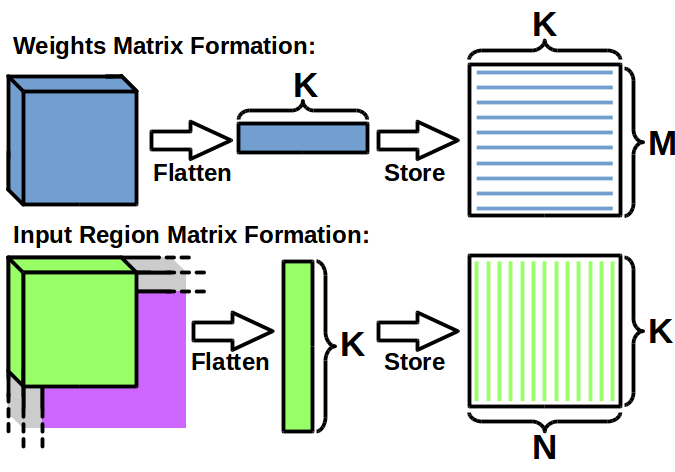
\includegraphics[width=0.75\textwidth]{../figures/im2col.png}
\caption{A visualisation of the reshaping process. The weights data is shown in blue, and the input region data is shown in green, embedded in a purple feature map with grey padding} \label{fig:im2col}
\end{figure}

In this approach, the weights kernels are considered to be three dimensional, where the height and width are given by the kernel size, and the depth is given by the depth of the input feature map. The each three-dimensional weights kernel is flattened into a row and the each row is stored sequentially. Thus the result is an $MxK$ matrix where $M$ is the number of weights kernels, and $K$ is the volume of an individual kernel. If the weights are stored sequentially in memory in the right order, this reshaping process can be done without copying any data to new locations. In such conditions, it is a simple case of setting the dimensions of the weights blob, thereby changing how the memory will be accessed.

Then the input feature map is considered in terms of input regions, i.e. each area that will be multiplied with weights kernels. The size of these regions matches the weights kernel, and the number is dependent on the input size, kernel size, padding and stride.  These input regions are flattened and stored as columns. However, this is not as simple as reshaping the blobs. If the convolution has padding, the input regions may contain extra zeros. Additionally, the stride and kernel size may result in input regions are overlapping or are not continuous. Therefore, each input region is individually mapped and copied from the input data into columns. This forms a $KxN$ matrix, where $K$ is the volume of an input region, and $N$ is the number of input regions in the input feature map.

The output of the convolution is then found with \( \mathbf{C} = \mathbf{A}\times\mathbf{B}\), where $\mathbf{C}$ is the output matrix, $\mathbf{A}$ is the weights matrix, and $\mathbf{B}$ is the matrix of input regions. In order for this computation to be valid, it should be clear that the volume of an input region is the same as the volume of a kernel. The $MxN$ output matrix can be treated as blob with depth $M$, equal to the number of weights, and width and height that give a product $N$, equal to the number of input regions.

By reducing the convolution to a single matrix multiplication, the algorithm can take advantage of a software library called Basic Linear Algebra Subprograms, or BLAS. This can bring significant performance improvements, as the BLAS library can provide highly optimised functions for a given platform. One such function is called \lstinline|gemm()|, and performs a general matrix multiplication. To be precise, gemm \lstinline|gemm()| performs $\mathbf{C} \gets \alpha\mathbf{A}\mathbf{B} + \beta\mathbf{C}$, where $\alpha$ and $beta$ are constants. By setting $\alpha = 1$ and $beta = 0$, the \lstinline|gemm()| function can be used to compute the output of the convolution. This method is therefore ideal for a software implementation of the convolution, but is not suitable for 

\subsubsection{Pure Convolution Method}
\label{sec:Imp-Layers-Conv-PC}
\vspace{-12pt}
Directly interpreting the convolution algorithm as described in \ref{sec:Background-CNN-Conv}, the pseudocode in Code \ref{code:conv-initial} can be formed. This code iterates through the rows, columns and depth layers of the output, as well as the rows and columns of the weights kernels and the depth layers of the input. The input row and column for the given kernel and output locations are found in lines 6 and 8. These are used to check whether the input location is in padding, which causes no change to the output. If the input location is not within a padded region, the value in the output feature map is incremented by the product of the corresponding weight and input values.

\renewcommand{\lstlistingname}{Code}
\begin{lstlisting}[frame=single, caption=Basic Convolution, label=code:conv-initial, captionpos=b, numbers=left, language=C]
for(outRow = 0; outRow < OutputWidth; outRow++) {
  for(outCol = 0; outCol < OutputlHeight; outCol++) {
    for(outDepth = 0; outDepth < OutputDepth; outDepth++) {
      for(inDepth = 0; inDepth < InputDepth; inDepth++) {
        for(kernelRow = 0; kernelRow < KernelRows; kernelRow++) {
          inRow = stride * outRow + kernelRow - pad;
          for(kernelCol = 0; kernelCol < KernelCols; kernelCol++) {
            inCol = stride * outCol + kernelCol - pad;
            if((0 <= inRow < InputHeight) &&  (0 <= inCol < InputWidth)) {
              output[outDepth][outRow][outCol] +=
                weights[outDepth][inDepth][kernelRow][kernelCol] *
                input[inDepth][inRow][inCol];
}}}}}}}
\end{lstlisting} 



\begin{itemize}
\item Describe layer code, including use of gemm function
\item Explain redesign, benefits of zhang implementation over im2col and gemm
\item tiled approach and optimizations
\end{itemize}

\subsubsection{Fully Connected Layer}
\label{sec:Imp-Layers-FC}
\vspace{-12pt}

\begin{itemize}
\item Describe layer code
\item Explain FC->CONV conversion
\item Explain redesign, benefits of new implementation
\end{itemize}

\subsubsection{Rectified Linear Unit Layer}
\label{sec:Imp-Layers-Relu}
\vspace{-12pt}

\begin{itemize}
\item Describe layer code
\end{itemize}

\subsubsection{Pooling Layer}
\label{sec:Imp-Layers-Pool}
\vspace{-12pt}

\begin{itemize}
\item Describe layer code
\end{itemize}

\subsubsection{Softmax Layer}
\label{sec:Imp-Layers-Prob}
\vspace{-12pt}

\begin{itemize}
\item Describe layer code
\end{itemize}

\subsection{Hardware Optimisations}
\label{sec:Imp-Optimisations}
\vspace{-12pt}

\begin{itemize}
\item Describe optimisations performed with HLS, i.e. pipelining, partitioning arrays, etc
\end{itemize}

\newpage

\section{Testing}
\label{sec:Test}
\vspace{-12pt}

The focus of this section is on the verification methods used to confirm that the system implementation was correct. The testing methods for individual layers will be analysed first, followed by tests for the whole network.

\subsection{Layer Testing}
\label{sec:Test-Layers}
\vspace{-12pt}

\begin{itemize}
\item Describe test functions for layers
\item Describe comparison to pure C++ implementation
\end{itemize}

\subsection{Network Testing}
\label{sec:Test-Network}
\vspace{-12pt}

\begin{itemize}
\item Describe test functions for Network
\item Describe comparison to pure C++ implementation
\end{itemize}

\newpage

\section{Evaluation}
\label{sec:Eval}
\vspace{-12pt}

\begin{itemize}
\item Summarise project specification requirements, and evaluate success on each
\end{itemize}

\subsection{FPGA Implementation of a CNN}
\label{sec:Eval-FPGAImplOfCnn}
\vspace{-12pt}

\begin{itemize}
\item How much of CNN was implemented
\item Hardware resources used
\item CNN performance
\item Layer computation time
\end{itemize}

\subsection{Fault Tolerance Investigation}
\label{sec:Eval-FaultTolInv}
\vspace{-12pt}

\begin{itemize}
\item Describe implementation of data collection, i.e. SocDrawer, test scripts, data collection scripts, etc
\item Analysis of data
\end{itemize}

\newpage

\section{Conclusion and Future Work}
\label{sec:Conclusion}
\vspace{-12pt}

\begin{itemize}
\item Summary of report sections
\item Summary of results and conclusion
\item Suggestions for future investigations
\end{itemize}

\newpage

\bibliography{finalReport_ref}
\bibliographystyle{ieeetr}
\nocite{*}


\end{document}